% **************************************************
% Macro specifiche per il documento corrente
% **************************************************
% Nome
\newcommand{\docName}{Specifica tecnica}
% Nome file
\newcommand{\docFileName}{specifica\_tecnica.1.0.pdf}
% Versione
\newcommand{\docVers}{0.1}
% Data creazione
\newcommand{\creationDate}{2013-01-16}
% Data ultima modifica
\newcommand{\modificationDate}{2013-01-17}
% Stato in {Approvato, Non approvato}
\newcommand{\docState}{Non approvato}
% Uso in {Interno, Esterno}
\newcommand{\docUsage}{Interno}
% Destinatari da specificare come nome1\\ &nome2\\ ecc.
\newcommand{\docDistributionList}{Team SoftwareSynthesis}
% Redattori da specificare come nome1\\ &nome2\\ ecc.
\newcommand{\docAuthors}{}
% Approvato da
\newcommand{\approvedBy}{}
% Verificatori
\newcommand{\verifiedBy}{}
% Perscorso (relativo o assoluto) che punta alla directory contenente shared/
% come sua sottodirectory (per comodità chiamiamola 'doc root').
\newcommand{\docRoot}{..}
% definire se si vuole l'indice delle tabelle
\def\INDICETABELLE{false}
% definire se si vuole l'indice delle figure
\def\INDICEFIGURE{false}

% importa il preambolo condiviso da tutti i documenti
% shared/preamble.tex
%
% Questo documento contiene la parte del preambolo condivisa e viene pertanto
% richiamato nel 'master' di tutti i documenti di progetto.  Al suo interno
% contiene le inclusioni (e le configurazioni) di tutti i package richiesti per
% la compilazione dei documenti, le macro di carattere generale e la definizione
% degli stili di pagina.

\documentclass[a4paper,10pt,openright]{article}

% **************************************************
% Macro generiche
% **************************************************
\newcommand{\team}{Software Synthesis}                    % chi siamo
\newcommand{\email}{software.synthesis@gmail.com}         % e-mail
\newcommand{\caName}{}                                    % titolo capitolato
\newcommand{\caDescr}{}                                   % descrizione
\newcommand{\inglese}[1]{\textit{#1}}

% **************************************************
% Codifica e lingua dei documenti
% **************************************************
\usepackage[utf8x]{inputenc}                              % codifica caratteri dei documenti sorgenti
\usepackage[english,italian]{babel}                       % localizzazione ai fini di sillabazione e cross-references
\usepackage[T1]{fontenc}                                  % codifica font di output

% **************************************************
% Definizione geometria della pagina
% **************************************************
\usepackage[a4paper,head=4cm,top=4.5cm,bottom=3cm,left=3cm,right=3cm,bindingoffset=5mm]{geometry}

% *************************************************
% Intestazioni e piè di pagina personalizzati
% *************************************************
\usepackage{fancyhdr}
% stile normale
\fancypagestyle{normal}{
\fancyhead{}                                              % intestazione
\fancyhead[RE,RO]{
\begin{picture}(0,0)
  \put(-410,0){
\includegraphics[width=1.02\textwidth]{header_logo}}
  \put(-410,10){\sffamily\large\leftmark}
\end{picture}
\vspace{-4pt}
}
\renewcommand{\headrulewidth}{.4pt}                       % riga sotto l'intestazione
\cfoot{}                                                  % piè di pagina
\fancyfoot[RO,LE]{\sffamily
  pag.~\thepage{} di \pageref{LastPage}}                  % a dx nelle pag. dispari e a sx in quelle pari
\fancyfoot[RE,LO]{\sffamily\docFileName{} -- v.\docVers}
\renewcommand{\footrulewidth}{.4pt}                       % riga sopra il piè di pagina
}
% stile per gli indici
\fancypagestyle{toc}{
\fancyhead{}                                              % intestazione
\fancyhead[RE,RO]{
\begin{picture}(0,0)
  \put(-410,0){
\includegraphics[width=1.02\textwidth]{header_logo}}
\end{picture}
}
\renewcommand{\headrule}{}                                % nessuna riga sotto l'intestazione
\cfoot{}                                                  % piè di pagina
\fancyfoot[RO,LE]{\sffamily\thepage{}}                    % a dx nelle pag. dispari e a sx in quelle pari
\fancyfoot[RE,LO]{\sffamily\docFileName{} -- v.\docVers}
\renewcommand{\footrulewidth}{.4pt}                       % riga sopra il piè di pagina
}

\pagestyle{fancy}                                         % premetto: non so usare bene le marche:
\renewcommand{\sectionmark}[1]{\markboth{#1}{#1}}         % se qualcuno ha idee migliori si faccia avanti!

% **************************************************
% Tabelle
% **************************************************
\usepackage{tabularx}                                     % tabelle di larghezza fissa con una o più colonne variabili
\usepackage{multirow}                                     % colonne con colonne che si estendono per più righe
\usepackage{booktabs}                                     % per inserire l'ambiente table e le righe orizz. nelle tabelle
\usepackage{longtable}			                          % tabelle oltre i limiti di pagina

% **************************************************
% Cross-references e collegamenti ipertestuali
% **************************************************
\usepackage[hidelinks]{hyperref}
\hypersetup{%
  colorlinks=false, linktocpage=false, pdfborder={0,0,0}, pdfstartpage=3, pdfstartview=FitV,%
  urlcolor=Cyan, linkcolor=Cyan, citecolor=Black, %pagecolor=Black,%
  pdftitle={\docName}, pdfauthor={\team}, pdfsubject={}, pdfkeywords={},%
  pdfcreator={pdflatex}, pdfproducer={pdflatex with hyperref package}%
}

% **************************************************
% Immagini e grafica
% **************************************************
\usepackage{graphicx}                                     % supporto ad aspetti avanzati delle immagini
\graphicspath{{\docRoot/pics/}}                           % percorso contenente tutti i file immagini
\usepackage{color}                                        % permette di colorare facilmente il testo

% **************************************************
% Altri pacchetti opzionali
% **************************************************     
\usepackage{lastpage}                                     % per sapere il numero totale di pagine
\usepackage{lipsum}                                       % genera "dummy text" per prove di impaginazione
\usepackage{eurosym}                                      % per il simbolo dell'euro usare \EUR{x} dove x è l'importo


% Fine del preambolo e inizio del documento
\begin{document}

% Inclusione della prima pagina
% shared/firstpage.tex
%
% Questo documento definisce il contenuto della prima pagina, che si suppone
% essere uguale in tutti i documenti.  Oltre al logo e al titolo, la prima
% pagina contiene i metadati relativi al documento in cui viene inclusa.


% rimuove intestazioni e piè di pagina
\pagestyle{empty}

\begin{center}

% logo del gruppo

\includegraphics[width=1.5\textwidth]{logo}

\vspace{1in}

% titolo del documento
{\Huge\bfseries \docName}

\vspace{1in}

% tabella riepilogativa
\begin{tabularx}{.7\textwidth}{>{\bfseries\sffamily}l>{\sffamily}l}
\toprule
\multicolumn{2}{>{\sffamily}c}{Informazioni sul documento}\\
\midrule
Nome file:            & \docFileName\\
Versione:             & \docVers\\
Data creazione:       & \creationDate\\
Data ultima modifica: & \modificationDate\\
Stato:                & \docState\\
Uso:                  & \docUsage\\
Redattori:            & \docAuthors\\
Approvato da:         & \approvedBy\\
Verificatori:         & \verifiedBy\\
\bottomrule
\end{tabularx}

\end{center}

\newpage


%---------------------------RUOLI----------------------------
%FASE 1:
%Progettisti: TRES, STEFANO, SCHIVO;
%FASE 2:
%Progettisti: DIEGO, ELENA, RIZZI

%Verificatore: Andrea Meneghinello
%Responsabile finale TRES
%------------------------------------------------------------

% Storico delle modifiche
\section*{Storia delle modifiche}
\begin{center}
\begin{longtable}{lp{.32\textwidth}lll}
\toprule
Versione & Descrizione intervento & Membro & Ruolo & Data\\
\midrule % inserire qui il contenuto della tabella
0.2 & Stesura dell'introduzione ai design pattern. Stesura dell'introduzione ai tracciamenti. & Stefano Farronato & Progettista & 2013-01-17\\
0.1 & Creazione del documento e stesura della sezione ``Introduzione''. & Riccardo Tresoldi & Progettista & 2013-01-16\\
\bottomrule
\end{longtable}
\end{center}
\newpage

% inclusione dell'indice
% shared/toc.tex
%
% Questo file contiene le istruzioni che generano l'indice o gli indici del
% documento (utile nel caso in cui decidessimo di avere anche un indice delle
% tabelle e/o un indice delle figure).

\pagestyle{toc}
\pagenumbering{roman}

\tableofcontents

\newpage


% Alcuni aggiustamenti per le pagine
\pagenumbering{arabic}
\setcounter{page}{1}
\pagestyle{normal}

% Qui ha inizio il documento vero e proprio...

\newpage

\section{Introduzione}
\subsection{Scopo del prodotto}
\purpose

\subsection{Scopo del documento}
Il presente documento è stato redatto al fine di produrre le specifiche sulla progettazione ad alto livello, del prodotto MyTalk. A tal fine il documento presenterà:

\begin{itemize}
	\item Un elenco con le specifiche dei design pattern utilizzati.
	\item Una descrizione dettagliata dei componenti rilevati in fase di progettazione indicando il tipo,
la funzione e l'obbiettivo.
	\item L'architettura d'alto livello del sistema.
	\item I diagrammi UML per definire i flussi principali di controllo dell'applicativo.
	\item Il tracciamento dei requisiti e delle componenti, negli schemi: requisiti-componeneti e componenti-requisiti.
\end{itemize}

\subsection{Glossario}
\glossaryIntro

\clearpage
\section{Riferimenti}

\subsection{Normativi}
\begin{itemize}
\item[] \textit{piano\_di\_qualifica.2.0.pdf} allegato.
\item[] \textit{norme\_di\_progetto.2.0.pdf} allegato.
\item[] \textit{analisi\_dei\_requisiti.2.0.pdf} allegato
\end{itemize}

\subsection{Informativi}
\begin{itemize}
\item[] Capitolato d'appalto: \caName{}, v1.0, redatto e rilasciato dal proponente Zucchetti s.r.l. reperibile all'indirizzo \url{http://www.math.unipd.it/~tullio/IS-1/2012/Progetto/C1.pdf};
\item[] testo di consultazione: \textit{Software Engineering (8th edition) Ian Sommerville, Pearson Education | Addison Wesley};
\item[] manuale all'utilizzo dei design pattens: \textit{Design Patterns, Elementi per il riuso di software a oggetti - (1/Ed. italiana) Eric Gamma, Richard Helm, Ralph Johnson, John Vlissides, Pearson Education};
\item[] \textit{glossario.1.0.pdf} allegato.
\end{itemize}

\clearpage
\section{Design Pattern}
In questa sezione discuteremo i design pattern utilizzati nella progettazione delle componenti. Ogni desing pattern sarà proposto con la seguente forma:

\begin{itemize}
	\item \textbf{Scopo}: verrà proposto lo scopo generico del pattern, al fine di evidenziare subito la sua utilità.
	\item \textbf{Diagramma esemplificativo}: si riporterà lo schema UML, rappresentante un implementazione generica del design pattern in esame.
	\item \textbf{Vantaggi derivanti}: si darà un elenco dei vantaggi apportati dall'utilizzo del pattern, in particolare sotto il profilo della manutenzione e del riuso del codice.
	\item \textbf{Componenti che lo implementano}: infine verranno elencati i componenti dell'architettura di sistema, che implementano il pattern descritto.
\end{itemize}

Per una visione d'insieme dei delle componenti utilizzate da un pattern, e dei pattern utilizzati da un componente, rimandiamo alle sottosezioni ``Tracciamenti Componenti-Design Pattern'' e ``Tracciamenti Design Pattern-Componenti'' della sezione ``Tracciamenti''.

%\subsection{Template descrizione design pattern}
%\subsubsection{Scopo}
%\subsubsection{Diagramma esemplificativo}
%\subsubsection{Vantaggi derivanti}
%\begin{itemize}
%\item
%\item
%\end{itemize}
%\subsubsection{Componenti che lo implementano}

\subsection{Adapter}
\subsubsection{Scopo}
Convertire l'interfaccia di una classe in un altra interfaccia richiesta dal \underline{client} e consente a classi diverse di operare insieme quando ciò non sarebbe altrimenti possibile a causa di interfacce incompatibili.
\subsubsection{Diagramma esemplificativo}
\subsubsection{Vantaggi derivanti}
\begin{itemize}
\item consente di adattare una classe esistente senza doverla ridefinire;
\item un unico oggetto può adattare più classi.
\end{itemize}
\subsubsection{Componenti che lo implementano}

\subsection{Composite}
\subsubsection{Scopo}
Il pattern Composite ha lo scopo di comporre oggetti in strutture ad albero al fine di rappresentare gerarchie parte-tutto e consentire ai \underline{client} di trattare oggetti singoli e composizioni in modo uniforme. Permette inoltre di gestire strutture dati gerarchicizzate con elementi "foglie" ed elementi "contenitori", l'ideale per la struttura "gruppo" e "utente".
\subsubsection{Diagramma esemplificativo}
\subsubsection{Vantaggi derivanti}
\begin{itemize}
\item definisce gerarchie di classi costituite da oggetti primitivi e composti;
\item semplifica il \underline{client} in quanto posso trattare oggetti singoli e strutture astratte in modo uniforme;
\item rende più semplice l'aggiunta di nuovi componenti.
\end{itemize}
\subsubsection{Componenti che lo implementano}

\subsection{Data Access Object (DAO)}
\subsubsection{Scopo}
Il pattern DAO ha lo scopo di disaccoppiare la logica di business dalla logica di accesso ai dati. Questo si ottiene spostando la logica di accesso ai dati dai componenti di business ad una classe DAO rendendo i componenti che implementano la logica di business indipendenti dalla natura del dispositivo di persistenza. Questo approccio garantisce che un eventuale cambiamento del dispositivo di persistenza non comporti modifiche sui componenti di business.
\subsubsection{Diagramma esemplificativo}
\subsubsection{Vantaggi derivanti}
\begin{itemize}
\item stratifica e isola l'accesso ad una tabella dalla parte di business logic;
\item crea un maggiore livello di astrazione;
\item mantiene una rigida separazione tra le componenti di un'applicazione (Model - Controller).
\end{itemize}
\subsubsection{Componenti che lo implementano}

\subsection{Factory Method}
\subsubsection{Scopo}
Definisce un'interfaccia per la creazione di un oggetto, lasciando alle sottoclassi la decisione sulla classe che deve essere istanziata e consente di deferire l'istanziazione di una classe alle sottoclassi.
\subsubsection{Diagramma esemplificativo}
\subsubsection{Vantaggi derivanti}
\begin{itemize}
\item fornisce un punto di aggancio per le sottoclassi per la produzione di una versione specializzata di un oggetto;
\item connette gerarchie di classi parallele;
\end{itemize}
\subsubsection{Componenti che lo implementano}

\subsection{Façade}
\subsubsection{Scopo}
Fornire un interfaccia unificata per un insieme di interfacce presenti in un sottosistema. Façade definisce un interfaccia di livello più alto che rende il sottosistema più semplice da utilizzare.
\subsubsection{Diagramma esemplificativo}
\subsubsection{Vantaggi derivanti}
\begin{itemize}
\item nasconde ai \underline{client} i componenti del sottosistema rendendo quest'ultimo più facile da usare;
\item promuove l'accoppiamento lasco tra un sottosistema e i \underline{client}, ossia consente di modificare i componenti del sottosistema senza che i suoi \underline{client} siano coinvolti.
\end{itemize}
\subsubsection{Componenti che lo implementano}

\subsection{Model-View-Presenter}

\subsubsection{Scopo}
Il pattern architetturale \foreignlanguage{english}{Model-View-Presenter} similmente a quanto accade per \foreignlanguage{english}{Model-View-Controller} (MVC), ha lo scopo di mantenere separata la \textit{business logic}, cioè la gestione dei dati secondo le regole di un determinato dominio e la loro memorizzazione in forma persistente, dalla presentazione e manipolazione mediante interfaccia utente.

\subsubsection{Diagramma esemplificativo}
\begin{figure}[h]
\centering
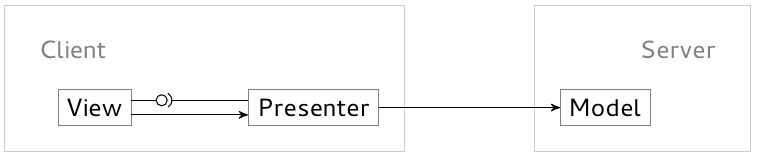
\includegraphics[width=.7\textwidth]{mvpHLdiagram}
\caption{Diagramma ad alto livello del pattern MVP.}\label{fig:mvpHL}
\end{figure}


\subsubsection{Vantaggi derivanti}
\begin{itemize}
\item riduce l'accoppiamento fra le componenti del sistema permettendo, ad esempio, di modificare la grafica (View) senza dover per questo preoccuparsi delle operazioni di aggiornamento dei dati;
\item computazione lato \underline{client}, quindi per tutte le operazioni che non coinvolgono direttamente il modello non è necessario appoggiarsi alla connessione di rete in quanto tutti i dati e la logica necessaria sono già disponibili sul \underline{client}.
\end{itemize}

\subsubsection{Componenti che lo implementano}

\subsection{Singleton}

\subsubsection{Scopo}
Il pattern creazionale Singleton, garantisce che una determinata classe possa essere istanziata una sola volta, e di fornirne un punto di accesso globale. Questo pattern va utilizzato negli ambiti in cui si ha la necessità che l'accesso ad una determinata entità sia unico, in modo da permettere la gestione ottimale della risorsa stessa.

\subsubsection{Diagramma esemplificativo}
\begin{figure}[h]
\centering
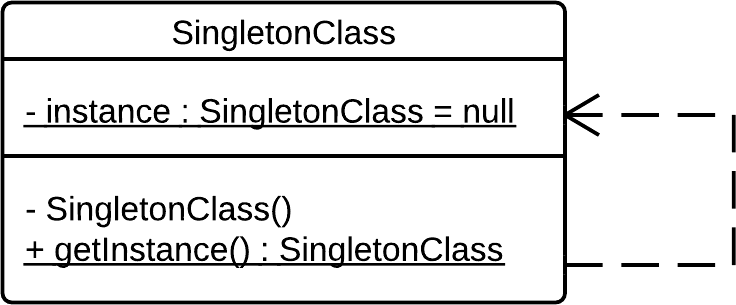
\includegraphics[width=.7\textwidth]{singletonHLdiagram}
\caption{Diagramma ad alto livello del pattern Singleton.}\label{fig:singletonHL}
\end{figure}

\subsubsection{Vantaggi derivanti}
\begin{itemize}
\item accesso controllato a un'unica istanza;
\item riduzione dello spazio dei nomi in quanto riduce l'uso di variabili globali;
\item permette di gestire un numero variabile di istanze.
\end{itemize}

\subsubsection{Componenti che lo implementano}

\subsection{State}
\subsubsection{Scopo}
Permette ad un oggetto di cambiare il suo comportamento al variare del suo stato interno, quindi a run-time. L'oggetto si comporterà come se avesse cambiato la sua classe.
\subsubsection{Diagramma esemplificativo}
\begin{figure}[h]
\centering
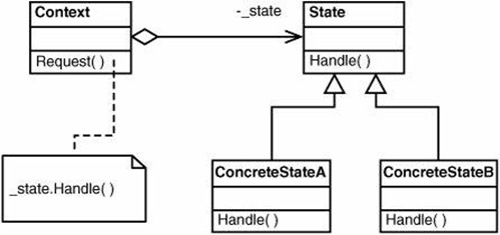
\includegraphics[width=.8\textwidth]{DesignPatternState}
\caption{Diagramma ad alto livello del pattern State.}\label{fig:state}
\end{figure}
\subsubsection{Vantaggi derivanti}
\begin{itemize}
\item specializza il comportamento associato ad uno stato;
\item rende esplicita la transazione si stato (tale condizione è espressa esplicitamente);
\item condivisione di oggetti di stato.
\end{itemize}

\subsubsection{Componenti che lo implementano}







\subsection{Strategy}
\subsubsection{Scopo}
Ha lo scopo di definire degli algoritmi, incapsularli e renderli intercambiabili. Permette inoltre agli algoritmi di variare indipendentemente dai \underline{client} che ne fa uso.
\subsubsection{Diagramma esemplificativo}
\subsubsection{Vantaggi derivanti}
\begin{itemize}
\item famiglie di algoritmi correlati;
\item può essere usato al posto dell'ereditarietà
\item può essere un'alternativa ai blocchi di scelta condizionale per determinare il comportamento desiderato;
\item può fornire più implementazioni diverse dello stesso comportamento;
\end{itemize}
\subsubsection{Componenti che lo implementano}

\clearpage
\section{Introduzione all'architettura di sistema}

\clearpage
\section{Architettura MyTalk-Server}

\subsection{Componenti evidenziate}

\subsubsection{Template della componente X}
\begin{description}
	\item{\scshape\bfseries Descrizione:} 
	\item{\scshape\bfseries Diagramma del package:}
	\item{\scshape\bfseries Classi utilizzate:} 
\end{description}

\subsection{Classi utilizzate}

\subsubsection{Template classe X}
\begin{description}
	\item{\scshape\bfseries Descrizione:} 
	\item{\scshape\bfseries Diagramma della classe:}
	\item{\scshape\bfseries Componenti che ne fanno uso:} 
\end{description}

\subsection{Diagramma del package}

\subsection{Diagramma delle classi}
\clearpage

\section{Architettura MyTalk-client Universale}

\subsection{Componenti evidenziate}

\subsubsection{Template della componente X}
\begin{description}
	\item{\scshape\bfseries Descrizione:} 
	\item{\scshape\bfseries Diagramma del package:}
	\item{\scshape\bfseries Classi utilizzate:} 
\end{description}

\subsection{Classi utilizzate}

\subsubsection{Template classe X}
\begin{description}
	\item{\scshape\bfseries Descrizione:} 
	\item{\scshape\bfseries Diagramma della classe:}
	\item{\scshape\bfseries Componenti che ne fanno uso:} 
\end{description}

\subsection{Diagramma del package}

\subsection{Diagramma delle classi}
\clearpage

\section{Architettura MyTalk-clientSoftwareSynthesis}

\subsection{Componenti evidenziate}

\subsubsection{Template della componente X}
\begin{description}
	\item{\scshape\bfseries Descrizione:} 
	\item{\scshape\bfseries Diagramma del package:}
	\item{\scshape\bfseries Classi utilizzate:} 
\end{description}

\subsection{Classi utilizzate}

\subsubsection{Template classe X}
\begin{description}
	\item{\scshape\bfseries Descrizione:} 
	\item{\scshape\bfseries Diagramma della classe:}
	\item{\scshape\bfseries Componenti che ne fanno uso:} 
\end{description}

\subsection{Diagramma del package}

\subsection{Diagramma delle classi}
\clearpage

\section{Conclusioni sull'architettura}

\subsection{Diagrammi delle attività}

\subsection{Diagrammi di sequenza}
\clearpage

\section{Tracciamenti}
Nella seguente sezione vengono proposti tutti i tracciamenti eseguiti mediante il sistema Synthsis Requirment Manager. I tracciamenti proposti sono giustificati dalle seguenti due motivazioni:

\begin{itemize}
	\item Dimostrare il soddisfacimento per necessarietà e sufficienza della corrispondenza tra gli elementi tracciati (e.g. una componente deve rispondere necessariamente alle esigenze di uno o più requisiti, tali insomma che ne giustifichino l'esistenza. D'altro canto è richiesto che ogni requisito definito in fase d'analisi sia soddisfatto e risolto da almeno una componente).
	\item dare una lettura generale delle varie: componenti, requisiti, design pattern e classi.
\end{itemize}

\subsection{Tracciamenti Requisiti-Componenti}

\subsection{Tracciamenti Componenti-Requisiti}

\subsection{Tracciamenti Componenti-DesignPattern}

\subsection{Tracciamenti DesignPattern-Componenti}

\subsection{Tracciamenti Componenti-Classi}

\subsection{Tracciamenti Classi-Componenti}

\end{document}